%-----------------------------------------------------------------------------
%\begin{itemize}
%	\item Học tăng cường kết hợp với học sâu
%		\begin{itemize}
%			\item Giới thiệu học sâu
%			\item Mạng nơ-ron tích chập
%			\item Sử dụng mạng nơ-ron để xấp xỉ hàm
% 			\item Học tăng cường kết hợp với xấp xỉ hàm
%		\end{itemize}
%
%	\item Kết hợp học tăng cường với học sâu vào bài toán tự động chơi game
%		\begin{itemize}
%			\item Kỹ thuật làm tăng tính ổn định
%			\item Vấn đề ``overestimation'' của thuật toán Q-learning
%		\end{itemize}
%\end{itemize}
%-----------------------------------------------------------------------------

\chapter{Kết hợp học tăng cường với học sâu}
\ifpdf
\graphicspath{{Chapter3/Chapter3Figs/PNG/}{Chapter3/Chapter3Figs/PDF/}{Chapter3/Chapter3Figs/}}
\else
\graphicspath{{Chapter3/Chapter3Figs/EPS/}{Chapter3/Chapter3Figs/}}
\fi
\begin{quote}
\textit{Những thành công gần đây của học sâu (Deep learning) trong các bài toán như xử lý ngôn ngữ tự nhiên, nhận diện đối tượng trong ảnh... đặt ra vấn đề: liệu các kỹ thuật trong học sâu có thể áp dụng vào học tăng cường?
Để trả lời câu hỏi đó, chương này trình bày về hướng tiếp cận kết hợp học tăng cường với học sâu để áp dụng vào bài toán tự động chơi game. 
Hướng tiếp cận này giúp cho các thuật toán học tăng cường được trình bày trong chương 2 có thể áp dụng vào những bài toán thực tế với số lượng trạng thái rất lớn.
Chương này trình bày hai phần:
\begin{itemize}
	\item Các kiến thức cơ bản của học sâu và cách kết hợp học tăng cường với học sâu.
	\item Áp dụng hướng tiếp cận này vào bài toán tự động chơi game.
\end{itemize}}
\end{quote}

%-----------------------------------------------------------------------------
%-----------------------------------------------------------------------------
\section{Kết hợp học tăng cường với học sâu}

%-----------------------------------------------------------------------------
\subsection{Học sâu}
\subsubsection*{Lý do cần áp dụng học sâu}
	Những thuật toán học tăng cường được trình bày trong chương trước đều tìm chính sách tối ưu dựa vào hàm giá trị. 
	Việc tính \textbf{đúng} và \textbf{nhanh} hàm giá trị ảnh hưởng rất nhiều đến kết quả của bài toán. 
	Các thuật toán học tăng cường cổ điển như ``Monte Carlo'' (MC) hay ``Temporal-Difference'' (TD) đều đã được chứng minh là luôn hội tụ trong những điều kiện nhất định \cite{sutton1998introduction}. 
	Ngoài ra, khi áp dụng vào các bài toán kinh điển của học tăng cường thì các thuật toán này đều hội tụ khá nhanh.
	
	Tuy nhiên, với những bài toán thực tế với số trạng thái rất lớn thì việc lưu véc-tơ hàm giá trị trạng thái $v_{\pi}$ (hoặc ma trận hàm giá trị hành động $q_{\pi}$) là việc không thể. 
	Ví dụ như frame hình của bài toán tự động chơi game có kích thước $210\times160\times3=100800$ điểm ảnh; mỗi điểm ảnh có giá trị trong khoảng $[0, 127]$ nên số trạng thái có thể có lên đến $128^{100800}$.
	Vì vậy, việc lưu trữ hàm giá trị dưới dạng bảng là không khả thi về mặt bộ nhớ.
	Còn về mặt tốc độ tính toán thì các thuật toán học tăng cường trên đều tính hàm giá trị \textbf{rời rạc} cho từng trạng thái.
	Với số trạng thái quá lớn như trên thì ta không thể duyệt lần lượt từng trạng thái để tính được.
	
	Những lý do trên dẫn đến việc sử dụng một phương pháp xấp xỉ hàm là bắt buộc cho các bài toán học tăng cường với số trạng thái lớn.
	Một trong những tiếp cận rất tự nhiên đó là sử dụng các mô hình học có giám sát như là một phương pháp xấp xỉ hàm giá trị.
	Đặc biệt, với những đột phá gần đây của học sâu trong lĩnh vực xử lý ảnh, video... \cite{lecun2015deep} thì việc áp dụng các mô hình phổ biến của học sâu vào bài toán tự động chơi game là đầy hứa hẹn.
	
%-----------------------------------------------------------------------------
\subsubsection*{Giới thiệu học sâu}
	Các mô hình truyền thống trong lĩnh vực máy học như ``Linear regression'', ``Bayesian learning''... thông thường đều hoạt động trên các biểu diễn dữ liệu (thường được gọi là đặc trưng) được \textbf{rút trích một cách thủ công} (hand-designed features).
	Với dữ liệu thô thu thập được từ thực tế, các nhà khoa học xây dựng các phương pháp rút trích ra những ``thông tin hữu ích'' để cung cấp cho các mô hình máy học.
	Kết quả nhận được từ các mô hình này phụ thuộc rất lớn vào cách biểu diễn dữ liệu.
	Ví dụ như trong bài toán nhận diện người nói từ một đoạn âm thanh, các đặc trưng có thể bao gồm: độ lớn âm thanh, tần số trung bình của đoạn âm,...
	Nếu các đặc trưng này không đủ ``tốt'' (như có hai người nói đoạn âm thanh nhưng lại có chung độ lớn, tần số...) thì các mô hình học sẽ không thể phân biệt.
		
	Để giải quyết vấn đề thiết kế đặc trưng, các mô hình máy học thuộc loại ``Học biểu diễn'' \textit{(Representation learning)} ra đời.
	Các mô hình này có khả năng tự động học luôn các đặc trưng cần thiết cho quá trình phân tích dữ liệu.
	Nhờ vậy, các mô hình này có thể áp dụng được dễ dàng hơn vào các bài toán thực tế mà không cần con người phải can thiệp.
	Tuy nhiên, các đặc trưng cần thiết lại có thể rất phức tạp.
	Việc học ra các đặc trưng này có thể khó ngang với việc giải bài toán gốc.
	Ví dụ như trong bài toán nhận diện người nói trên, ta có thể sử dụng thông tin về giọng địa phương (accent) của người nói.
	Đặc trưng này rất trừu tượng, không dễ phân tích bằng máy tính mặc dù con người có thể nhận biết một cách khá dễ dàng.
	Vì vậy, nếu các đặc trưng cần thiết quá khó để học thì các mô hình máy học thuộc loại ``Học biểu diễn'' cũng không thể cho kết quả tốt.

	Học sâu (Deep learning) được ra đời nhằm giải quyết các vấn đề trên.
	Học sâu là một nhánh của ``Học biểu diễn'' nên vẫn có thể tự động học ra các đặc trưng hữu ích.
	Học sâu được thiết kế để học ra các đặc trưng có quan hệ với nhau theo nhiều tầng (layer).
	Các đặc trưng ở tầng phía sau được xây dựng dựa vào các đặc trưng ở tầng phía trước.
	Các tầng đầu tiên bao gồm những đặc trưng đơn giản và các tầng tiếp theo ngày càng trừu tượng, ngày càng phức tạp hơn.
	Mỗi tầng chỉ cần học cách xây dựng đặc trưng từ những đặc trưng ở tầng phía trước (đã có sẵn độ trừu tượng nhất định) thay vì học từ dữ liệu thô ban đầu; điều này giúp cho học sâu có khả năng học được những đặc trưng có tính trừu tượng cao.
	
	\begin{figure}
		\centering
		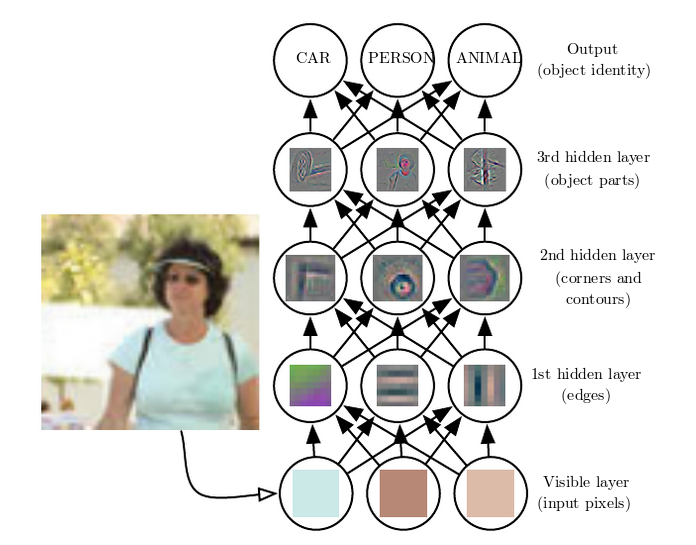
\includegraphics[width=\textwidth]{deep_learning_example}
		\label{fig_dl_Example}
		\caption[Hình mô phỏng cách hoạt động của mô hình học sâu]{Hình mô phỏng cách hoạt động của mô hình học sâu cho bài toán nhận diện đối tượng trong ảnh.
		Dữ liệu đầu vào là hình ảnh RGB chứa đối tượng cần xác định. Tầng đầu tiên của mô hình là tầng input tiếp nhận thông tin này dưới dạng ma trấn số. 
		Các tầng tiếp theo ngoại trừ tầng cuối cùng được gọi là tầng ẩn ``hidden layer'' vì đặc trưng học được tại đây con người không quan sát được. 
		Các tầng ẩn học các đặc trưng ngày càng trừu tượng dựa vào đặc trưng ở tầng phía trước. 
		Tầng ẩn đầu tiên học được các đặc trưng về cạnh bằng cách so sánh độ sáng giữa các điểm ảnh gần nhau. 
		Tầng ẩn thứ hai học được các đặc trưng về đường cong bằng cách tổng hợp đặc trưng về cạnh ở tầng trước đó. 
		Tầng ẩn thứ ba học được các đặc trưng về bộ phận của đồ vật như khuôn mặt, bánh xe... dựa vào các đặc trưng về đường cong ở tầng trước. 
		Tầng cuối cùng được gọi là tầng output có nhiệm vụ tìm kiếm các bộ phận và trả về lớp đối tượng tương ứng. 
		Bằng cách học đặc trưng ngày càng trừu tượng hơn, các mô hình học sâu có khả năng tự động học được các đặc trưng từ đơn giản đến phức tạp; tất cả đều nhằm hỗ trợ cho quá trình phân lớp dữ liệu (hình được chỉnh sửa từ \cite{Goodfellow-et-al-2016-Book})}
	\end{figure}
	
	Một trong những mô hình học sâu phổ biến nhất và cũng cho kết quả rất tốt với dữ liệu ảnh \cite{lecun2015deep} đó là mạng nơ-ron tích chập (Convolutional Neural Networks).
	Với bài toán tự động chơi game, dữ liệu hệ thống nhận được từ môi trường là ảnh RGB.
	Chính vì vậy, mạng nơ-ron tích chập là một mô hình rất phù hợp để kết hợp với các thuật toán học tăng cường.
	
%-----------------------------------------------------------------------------
\subsection{Mạng nơ-ron tích chập}
	Mạng nơ-ron tích chập (Convolutional Neural Networks - CNN) là một mô hình học sâu được áp dụng rộng rãi trong các bài toán liên quan đến ảnh, video hoặc âm thanh... \cite{lecun2015deep}.
	CNN được thiết kế để tận dụng thông tin về không gian (spatial structures) của các loại dữ liệu nêu trên.
	Ví dụ như trong bài toán nhận diện mặt người trong ảnh, thông tin về vị trí của mắt, mũi, miệng,... là rất quan trọng.
	Nếu ta coi các điểm ảnh đều có ý nghĩa tương tự nhau thì ta đã bỏ quên thông tin về vị trí của những đặc trưng này.
	Trong khi đó, thông tin về vị trí tương đối của mắt, mũi, miệng... rõ ràng là rất quan trọng trong việc nhận diện mặt người.
	Trong ví dụ trên, nếu ta áp dụng các mô hình không quan tâm đến loại dữ liệu (coi từng thuộc tính dữ liệu đầu vào là độc lập) thì ta sẽ không tận dụng được thông tin về không gian trong đó.
	
	Để tận dụng thông tin về không gian trong dữ liệu ảnh, CNN được thiết kế để học các đặc trưng trên một vùng nhỏ của ảnh.
	Các đặc trưng này được lưu trữ dưới dạng những \textbf{bộ lọc} (filter) thường có \textbf{kích thước nh}ỏ hơn nhiều so với kích thước ảnh gốc.
	Các đặc trưng sau khi được học được áp dụng trên toàn bộ ảnh gốc để kiểm tra xem vị trí nào của ảnh xuất hiện đặc trưng này.
	CNN thực hiện phép kiểm tra này bằng cách ``trượt'' các bộ lọc này trên toàn bộ ảnh gốc.
	Phép ``trượt'' được thực hiện lần lượt từ trái qua phải và từ trên xuống dưới.
	Một cách tổng quát, phép ``trượt'' này có thể di chuyển không đồng đều theo hai chiều: ta có thể chỉ di chuyển qua phải một điểm ảnh nhưng lại di chuyển xuống dưới hai điểm ảnh.
	Tại mỗi vị trí, bộ lọc có nhiệm vụ kiểm tra thử đặc trưng được học có xuất hiện (hoặc mức độ rõ ràng của đặc trưng - đặc trưng xuất hiện nhiều hay ít) tại vị trí này không.
	Kết quả của phép kiểm tra này được lưu trữ lại dưới dạng một ``bức ảnh'' kết quả; giá trị mỗi ``điểm ảnh'' lúc này chính là kết quả của phép kiểm tra đặc trưng của bộ lọc.
	Do phép ``trượt'' được thực hiện theo thứ tự được nêu ở trên, các ``điểm ảnh'' kết quả vẫn mang thông tin tương đối về vị trí: ``điểm ảnh'' bên trái ứng với kết quả của vùng nằm bên trái trong ảnh gốc và tương tự với điểm ảnh bên phải.
	\begin{figure}
		\centering
		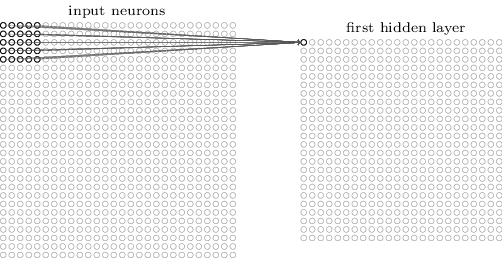
\includegraphics[width=.8\textwidth]{cnn_first_filter}
		\caption[Phép tính đặc trưng của CNN]{Hình mô tả phép ``kiểm tra'' đặc trưng của bộ lọc có kích thước $5\times5$ tại vị trí đầu tiên (góc trái trên) của ảnh đầu vào.
		Kết quả của phép ``kiểm tra'' này được lưu lại thành một ``điểm ảnh'' trong ``bức ảnh kết quả''.
		Lưu ý ảnh đầu vào trong ví dụ ở đây có kích thước $28\times28$.
		Do bộ lọc chỉ kiểm tra những vùng nằm hoàn toàn trong ảnh nên kích thước của ``bức ảnh'' đầu ra là $24\times24$.}
		\label{fig_cnn_filter}
		
		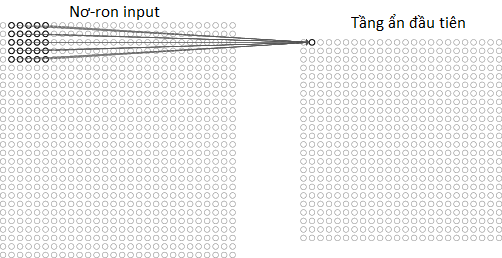
\includegraphics[width=.8\textwidth]{cnn_second_filter}
		\caption[Phép dịch chuyển bộ lọc của CNN]{Bộ lọc được trượt sang một điểm ảnh về phía bên phải để kiểm tra vùng cục bộ $5\times5$ bên cạnh.
		Kết quả của phép ``kiểm tra'' này được lưu lại thành một ``điểm ảnh'' bên phải của kết quả của vùng cục bộ trước đó.
		Thực hiện lần lượt quá trình ``trượt'' này đến hết ảnh ta sẽ có ``bức ảnh kết quả'' cuối cùng.
		``Bức ảnh kết quả'' này mang thông tin về một đặc trưng cụ thể tại những vùng cục bộ liên tiếp nhau trên ảnh gốc.}
		\label{fig_cnn_second_filter}	
	\end{figure}
	
	Phép ``kiểm tra'' đặc trưng của bộ lọc được thực hiện thông qua phép toán \textbf{tích chập} (convolution).
	Kết quả của phép tích chập được cộng với giá trị ``bias'' và đưa qua một hàm kích hoạt.
	Toàn bộ quá trình này có thể được biểu diễn thành công thức:
	\begin{equation}
		a_{i,j} = \sigma \left( b + \sum_{u = 0}^{height} \sum_{v = 0}^{width} w_{u, v} x_{i + u, j + v} \right)
	\end{equation}
	Trong đó:
	\begin{itemize}
		\item $a_{i,j}$ là kết quả của phép kiểm tra tại vùng có góc trái trên là $i, j$ trong ảnh gốc.
		\item $b$ là số thực gọi là ``bias'' của bộ lọc.
		\item $width, height$ lần lượt là chiều rộng và chiều cao của bộ lọc ($5\times5$ trong hình \ref{fig_cnn_filter}).
		\item $w$ là ma trận trọng số có kích thước $height \times width$ của bộ lọc. 
		$w_{u, v}$ là thành phần dòng $u$ cột $v$ của ma trận.
		\item $x_{i + u, j + v}$ là giá trị điểm ảnh đầu vào tại vị trí dòng $i + u$ và cột $j + v$.
		\item $\sigma$ là một hàm phi tuyến được gọi là hàm kích hoạt (activation function).
	\end{itemize}
	Phép toán tích chập này chỉ đơn giản là một tổng gồm các tích của trọng số và giá trị điểm ảnh.
	Hàm kích hoạt sau đó nhận kết quả của phép tích chập để thực hiện phép biến đổi phi tuyến tính; nhờ có hàm kích hoạt, bộ lọc có thể học được những đặc trưng phi tuyến tính.
	Một trong những hàm phi tuyến hay được áp dụng đó là hàm ``Rectified linear'': $\sigma(x)=\max(0, x)$.
	Công thức tích chập trên chứa hai thành phần cần được ``học'' đó là ``bias'' $b$ và ma trận trọng số $w$.
	Hai thành phần này lưu trữ thông tin về đặc trưng mà bộ lọc học được.
	Một trong những đặc điểm quan trọng nhất là việc ma trận trọng số $w$ và ``bias'' $b$ được sử dụng chung cho việc ``kiểm tra'' đặc trưng tại mọi vị trí của ảnh gốc (hình \ref{fig_cnn_second_filter}).
	Nhờ việc sử dụng chung ma trận trọng số và ``bias'' này, số lượng trọng số phải học của CNN được giảm đi rất nhiều.
	Cụ thể hơn, với ảnh gốc kích thước $28\times28 = 784$ như trong hình \ref{fig_cnn_filter}, nếu áp dụng mạng nơ-ron truyền thẳng thông thường để học đặc trưng từ toàn bộ ảnh, số lượng trọng số sẽ lên đến $784$ cho một đặc trưng.
	Trong khi đó, CNN chỉ gồm khoảng $5\times5=25$ trọng số cần học.
	
	Một bộ lọc của CNN chỉ học được một đặc trưng cụ thể.
	Tuy nhiên trong bài toán thực tế, ta cần nhiều đặc trưng khác nhau trên ảnh.
	Ví dụ như để nhận diện khuôn mặt trên ảnh, ta cần đặc trưng về mắt, miệng...
	Để học được nhiều đặc trưng khác nhau với CNN, ta chỉ việc thiết kế thêm nhiều bộ lọc học đặc trưng song song với nhau từ ảnh gốc.
	Với mỗi bộ lọc, ta cần học một ma trận trọng số và giá trị ``bias'' khác nhau.
	Ta gọi tập hợp các bộ lọc này là một tầng tích chập (convolution layer).
	Hình \ref{fig_cnn_layer} mô tả tầng tích chập với ba bộ lọc.
	\begin{figure}
		\centering
		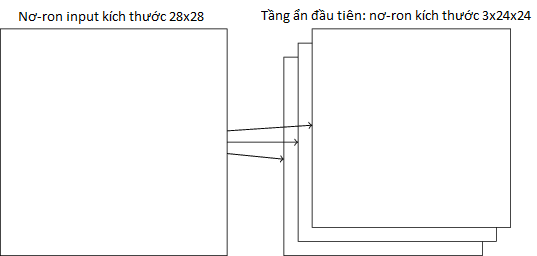
\includegraphics[width=.8\textwidth]{cnn_layer}
		\caption[Tầng tích chập với ba bộ lọc]{Hình mô tả tầng tích chập với ba bộ lọc học đặc trưng từ ảnh đầu vào.
		Mỗi bộ lọc lúc này học một bộ trọng số $w$ và giá trị ``bias'' $b$ khác nhau.
		Do các bộ lọc có cùng kích thước ($5\times5$) nên ``bức hình'' kết quả cũng có cùng kích thước.
		Ta coi mỗi ``bức hình'' kết quả như một kênh (channel) khác nhau của bức hình và ghép chúng lại thành một bức hình lớn hơn gồm ba kênh.
		Các kênh này cũng giống như ba kênh màu khác nhau của ảnh RGB.}
		\label{fig_cnn_layer}
	\end{figure}
	
	CNN là một mô hình học sâu.
	Vì vậy để học được những đặc trưng có tính trừu tượng cao, CNN áp dụng phương pháp tổng hợp đặc trưng trừu tượng từ những đặc trưng đơn giản hơn.
	Để tổng hợp đặc trưng, ta chỉ việc coi ``bức hình kết quả'' như là bức ảnh đầu vào và thêm tầng tích chập mới học đặc trưng từ bức hình này.
	Do kết quả của tầng tích chập trước mang thông tin về đặc trưng được học bởi các bộ lọc, tầng tích chập tiếp theo thực hiện việc học từ các đặc trưng đã học ở tầng trước.
	Nhờ vậy, việc thêm vào các tầng tích chập tiếp theo sẽ giúp mô hình học được những đặc trưng ngày càng trừu tượng hơn.
	
	Phần tiếp theo sẽ trình bày cách sử dụng CNN như là một công cụ xấp xỉ hàm hỗ trợ cho các thuật toán học tăng cường.
	Do có khả năng học đặc trưng tự động, ta có thể thiết kế một công cụ xấp xỉ hàm ``đa năng'': vừa học đặc trưng từ hình ảnh, vừa xấp xỉ hàm mong muốn từ những hình ảnh đó.

%-----------------------------------------------------------------------------
\subsection{Sử dụng mạng nơ-ron để xấp xỉ hàm}
	Việc sử dụng mạng nơ-ron để xấp xỉ hàm giá trị mang lại ba lợi ích quan trọng:
	\begin{itemize}
		\item Mạng nơ-ron có khả năng học được những đặc trưng phức tạp từ dữ liệu thô.
		\item Mạng nơ-ron có thể xấp xỉ hàm giá trị phức tạp.
		\item Mạng nơ-ron có thể tổng quát hoá từ trạng thái đã gặp sang trạng thái chưa gặp.
	\end{itemize}
	
	Mạng nơ-ron là một mô hình học sâu nên có thể học được những đặc trưng trừu tượng từ dữ liệu thô như đã nói ở phần trên.
	Cụ thể hơn trong bài toán tự động chơi game, ta có thể đưa dữ liệu đầu vào là các frame hình RGB thẳng vào input của mạng nơ-ron để tính ra giá trị tương ứng.
	Nhờ vậy, ta không cần phải thiết kế các đặc trưng bằng tay để biễu diễn lại từng trạng thái của game.
	Ngoài ra, do quá trình học đặc trưng là hoàn toàn tự động, thuật toán học tăng cường lúc này \textbf{có thể áp dụng cho bất kỳ game} nào mà không cần phải thay đổi cách rút trích đặc trưng.
	Với một mô hình cố định lúc này, ta có thể học chơi được nhiều game.
	Đây cũng chính là mục đích của bài toán tự động chơi game: xây dựng mô hình có khả năng tự động học chơi \textit{tốt} nhiều game chứ không chỉ chơi \textit{``hoàn hảo''} một game.
	
	Với bài toán tự động chơi game, giá trị của một trạng thái bất kỳ rất khó xác định do một màn game thường rất dài.
	Vì thế, \textbf{hàm giá trị của bài toán này là một hàm phi tuyến phức tạp} và không liên tục.
	Công cụ xấp xỉ hàm giá trị phải có khả năng xấp xỉ những hàm phức tạp như vậy thì thuật toán học tăng cường mới đạt được hiệu quả.
	Với cách nhìn nhận mạng nơ-ron như là một công cụ xấp xỉ hàm, ta có thể thấy mạng nơ-ron rất linh hoạt với khả năng xấp xỉ hàm đích bất kỳ.
	
	Một tính chất quan trọng khác của mạng nơ-ron chính là khả năng tổng quát hoá (generalization) từ trạng thái đã gặp sang trạng thái chưa gặp \cite{mnihdqn2015}.
	Nhờ đặc điểm này mà quá trình học được tăng tốc đáng kể.
	Thay vì phải duyệt qua từng trạng thái (thậm chí phải duyệt nhiều lần) để tính hàm giá trị tại đó, mạng nơ-ron có khả năng \textbf{``dự đoán'' giá trị} của một trạng thái chưa từng thấy dựa vào những trạng thái đã thấy.
	Như trong bài toán tự động chơi game thì các frame hình liên tiếp thường rất giống nhau và các trạng thái này thường cũng có giá trị tương đương nhau.
	Vì vậy, khi học xong cách chơi một game nào đó, hệ thống vẫn hoạt động tốt trong quá trình kiểm thử khi gặp những tình huống game chưa từng thấy trong lúc huấn luyện.
	
	Các thuật toán học tăng cường ở chương 2 đều lưu hàm giá trị dưới dạng bảng (lookup table).
	Để sử dụng mạng nơ-ron như một công cụ xấp xỉ hàm, lúc này ta coi hàm giá trị là một hàm có tham số (parameterized function) và đi tìm các tham số này:
	\begin{align}
		\hat{v}(s;\theta) &\approx v_{\pi}(s) \label{eq_DefVhat}\\
		\hat{q}(s,a;\theta) &\approx q_{\pi}(s,a) \label{eq_DefQhat}
	\end{align}
	$\theta$ là bộ trọng số của mạng nơ-ron mà ta cần học.
	Công thức (\ref{eq_DefVhat}) được dùng khi ta muốn xấp xỉ hàm giá trị trạng thái và công thức (\ref{eq_DefQhat}) là để xấp xỉ hàm giá trị hành động.
	Để học được bộ trọng số xấp xỉ tốt hàm đích ($v_{\pi}(s)$ hoặc $q_{\pi}(s,a)$), ta cung cấp các mẫu dữ liệu (data sample).
	Mỗi mẫu bao gồm dữ liệu đầu vào của mạng nơ-ron (tức trạng thái $s$ hoặc bộ trạng thái, hành động $s, a$) cùng với giá trị đích mong muốn (tức $v_{\pi}(s)$ hoặc $q_{\pi}(s,a)$).
	Khi ta cung cấp đủ nhiều mẫu dữ liệu cho mạng nơ-ron, các bộ tham số sẽ được thay đổi để mạng xấp xỉ được hàm đích mong muốn.
	Số lượng mẫu dữ liệu càng lớn thì mạng nơ-ron càng ``thấy'' được nhiều giá trị tại nhiều vị trí khác nhau của hàm đích hơn, khi đó mạng nơ-ron càng có khả năng xấp xỉ hàm đích tốt hơn.	
	Để xét xem mạng nơ-ron có xấp xỉ tốt hàm đích hay chưa, ta có thể tính độ ``khác biệt'' của giá trị đích với giá trị xấp xỉ trên cả không gian đầu vào:
	\begin{align}
		\label{eq_ExpectedErrorV}
		J(\theta) &= \mathbb{E}_{s \sim \pi}[(v_{\pi}(s) - \hat{v}(s;\theta))^2]\\
		\label{eq_ExpectedErrorQ}
		J(\theta) &= \mathbb{E}_{s,a \sim \pi}[(q_{\pi}(s,a) - \hat{q}(s,a;\theta))^2]
	\end{align}
	Kỳ vọng $\mathbb{E}_{s \sim \pi}$ ý chỉ kỳ vọng với biến ngẫu nhiên là trạng thái $s$ được lấy từ phân bố do chính sách $\pi$ tạo nên.
	Ví dụ như ta cần xấp xỉ hàm giá trị của một chính sách chỉ luôn ``đi qua trái'' thì $s$ sẽ là những trạng thái mà khi đi theo chính sách này, ta có thể gặp được $s$.
	Trong khi đó nếu chính sách đang xét là ``đứng yên'' (không thay đổi trạng thái) thì $s$ chỉ có thể có một trạng thái duy nhất đó là trạng thái bắt đầu.
	Giá trị nằm trong kỳ vọng là độ lỗi bình phương giữa giá trị xấp xỉ và giá trị đích.
	Với hàm lỗi bình phương, có thể thấy khi $J(\theta)$ càng nhỏ thì bộ trọng số $\theta$ giúp cho mạng nơ-ron xấp xỉ hàm đích càng tốt.
	Lý do chính ta chọn độ lỗi bình phương (ví dụ thay vì độ lỗi theo trị tuyệt đối) là vì việc tính toán (như đạo hàm) trên hàm bình phương dễ dàng hơn.
	
	Lưu ý là ở đây, hàm lỗi $J(\theta)$ là hàm theo $\theta$; tức là lúc này, ta cố định bộ trọng số $\theta$ để tìm ra ``sai số'' mà bộ trọng số này gây ra.
	Nếu ta có hai bộ trọng số $\theta_1$ và $\theta_2$, ta có thể so sánh khả năng xấp xỉ hàm đích của chúng bằng cách so sánh giá trị $J(\theta_1)$ và $J(\theta_2)$ tương ứng.
	
	Tuy nhiên ta không thể tính độ lỗi trên mọi điểm dữ liệu đầu vào theo công thức (\ref{eq_ExpectedErrorV}) và (\ref{eq_ExpectedErrorQ}) được vì số lượng trạng thái là rất lớn.
	Vậy ta có thể xấp xỉ giá trị $J(\theta)$ bằng cách chỉ xét độ lỗi trên một tập huấn luyện nhỏ (hay còn gọi là ``batch'') các trạng thái mà ta biết được giá trị đích.
	Khi đó, kỳ vọng $\mathbb{E}_{s \sim \pi}$ được thay thế bằng giá trị trung bình độ lỗi trên từng mẫu dữ liệu của ``batch'':
	\begin{align}
		\label{eq_BatchErrorV}
		J(\theta) &= \frac{1}{N} \sum_{i = 1}^{N}(v_{\pi}(S_{i}) - \hat{v}(S_{i};\theta))^2\\
		\label{eq_BatchErrorQ}
		J(\theta) &= \frac{1}{N} \sum_{i = 1}^{N}(q_{\pi}(S_i,A_i) - \hat{q}(S_i,A_i;\theta))^2		
	\end{align}
	Trong đó:
	\begin{itemize}
		\item N là số mẫu dữ liệu trong ``batch''.
		\item $S_i$, $A_i$ tương ứng là trạng thái và hành động của mẫu dữ liệu thứ $i$ của ``batch''.
	\end{itemize}
	Với một tập huấn luyện, ta mong muốn tìm được bộ trọng số giúp cho mạng nơ-ron xấp xỉ tốt hàm đích trên các mẫu dữ liệu thuộc tập huấn luyện này.
	Một thuật toán đơn giản và hay được sử dụng để tìm bộ trọng số này đó là ``Batch Gradient Descent'' (BGD).
	Để cực tiểu hoá hàm $J(\theta)$, thuật toán BGD thực hiện lặp lại nhiều ``bước đi'' nhỏ để thay đổi bộ trọng số $\theta$ dần dần; mỗi bước đi sẽ giúp cho hàm $J(\theta)$ giảm đi một ít.
	Để chọn ``hướng đi'' (tức cách cập nhật $\theta$) thì BGD sẽ ``nhìn'' xung quanh vị trí hiện tại và đi theo hướng nào giúp giảm $J(\theta)$ nhiều nhất có thể.
	Hướng đi này chính là ngược hướng véc-tơ đạo hàm riêng (tức ``gradient'') của hàm $J(\theta)$ tại $\theta$.
	Như vậy, thuật toán BGD thực hiện lặp lại nhiều lần việc cập nhật bộ trọng số $\theta$ theo công thức:
	\begin{equation}
		\theta_{t+1} = \theta_{t} - \alpha \nabla_{\theta}J(\theta)
	\end{equation}
	Trong đó:
	\begin{itemize}
		\item $\theta_{t}$ là bộ trọng số tại bước thứ $t$.
		\item $\alpha$ là hệ số học (learning rate); giá trị này dùng để điều khiển độ lớn của ``bước đi''.
		\item $\nabla_{\theta}J(\theta)$ là véc-tơ đạo hàm riêng của hàm $J(\theta)$ tại vị trí $\theta$.
	\end{itemize}
	Do ta chỉ ``nhìn'' cục bộ tại vị trí hiện tại nên nếu ta đi một bước quá dài (hệ số học $\alpha$ lớn) thì giá trị hàm lỗi $J$ tại điểm đến sẽ không chắc là luôn giảm;
	còn nếu bước đi quá ngắn thì mỗi bước chỉ giảm $J(\theta)$ một ít, khi đó ta sẽ tốn rất nhiều thời gian để $J(\theta)$ đạt giá trị cực tiểu.
	
	Một thuật toán cải tiến của BGD hay được sử dụng đó là ``Stochastic Gradient Descent'' (SGD).
	Điểm yếu của thuật toán BGD là ta cần phải tính véc-tơ đạo hàm riêng cho \textbf{tất cả} các mẫu trong ``batch'' để cập nhật được một lần cho bộ trọng số.
	Thuật toán SGD khắc phục điểm yếu này bằng cách chọn ngẫu nhiên một số mẫu dữ liệu trong ``batch'' (gọi là ``mini-batch''), tính véc-tơ đạo hàm riêng trung bình trên ``mini-batch'' này và thực hiện cập nhật bộ trọng số.
	Lúc này, véc-tơ đạo hàm riêng trung bình trên ``mini-batch'' có thể coi là một xấp xỉ của véc-tơ đạo hàm riêng trung bình trên toàn bộ tập huấn luyện.
	Do véc-tơ này chỉ tính trên ``mini-batch'' nên khi cập nhật, giá trị $J(\theta)$ có thể tăng.
	Tuy nhiên, khi cập nhật nhiều lần thì xu hướng chung là hàm lỗi $J(\theta)$ sẽ giảm.
	Khi tập huấn luyện càng lớn thì lợi thế của thuật toán SGD càng rõ.
	Với tập huấn luyện gồm 1000 mẫu thì thuật toán BGD chỉ cập nhật trọng số được \textbf{một} lần sau khi duyệt qua hết dữ liệu; trong khi đó, thuật toán SGD với kích thước ``mini-batch'' là 10 có thể cập nhật được 100 lần.
	Kích thước của ``mini-batch'' lúc này ảnh hưởng đến độ chính xác của véc-tơ đạo hàm riêng của $J(\theta)$.
	Nếu kích thước quá nhỏ thì véc-tơ đạo hàm riêng trung bình trên ``mini-batch'' sẽ không còn là một xấp xỉ tốt.
	Nếu kích thước quá lớn thì lợi thế về tốc độ của SGD so với BGD sẽ không còn cao.
	
	Như đã đề cập ở chương 2, để cải tiến chính sách khi không có đầy đủ thông tin về môi trường (tức không có các ma trận của MDP) ta cần xấp xỉ $q_{\pi}$ thay vì $v_{\pi}$. Áp dụng thuật toán SGD để cực tiểu hoá hàm lỗi (\ref{eq_BatchErrorQ}), công thức cập nhật bộ trọng số tại thời điểm $t$ có dạng:
	\begin{align}
		\theta_{t + 1} &= \theta_t - \Delta \theta_t \nonumber \\
		&= \theta_t - \alpha \nabla_{\theta_t} J(\theta_t) \nonumber \\
		&= \theta_t - \alpha \nabla_{\theta_t} \left( \frac{1}{B} \sum_{i = 1}^{B}(q_{\pi}(S_i,A_i) - \hat{q}(S_i,A_i;\theta_t))^2 \right) \nonumber\\
		\label{eq_SGDTrueQ_Update}
		&= \theta_t - \alpha \frac{1}{B} \sum_{i = 1}^{B}(q_{\pi}(S_i,A_i) - \hat{q}(S_i,A_i;\theta_t)) \nabla_{\theta_t} \hat{q}(S_i, A_i;\theta_t)
	\end{align}
	Ở đây:
	\begin{itemize}
		\item $\Delta \theta_t$ là giá trị cập nhật bộ trọng số $\theta_t$ với một ``mini-batch''.
		\item $B$ là kích thước của ``mini-batch''.
		\item $q_{\pi}(S_i,A_i)$ là giá trị \textbf{thật sự} của hành động $A_i$ tại trạng thái $S_i$.
		\item $\hat{q}(S_i,A_i;\theta_t)$ là giá trị \textbf{xấp xỉ} (với bộ trọng số $\theta_t$) của hành động $A_i$ tại trạng thái $S_i$.
		\item $\nabla_{\theta_t} \hat{q}(S_i, A_i;\theta_t)$ là véc-tơ đạo hàm riêng theo $\theta_t$ của hàm $\hat{q}$ tại trạng thái $S_i$ và hành động $A_i$.
	\end{itemize}
	Công thức trên bao gồm một tổng các số hạng có thể được tính riêng lẻ cho từng mẫu dữ liệu.
	Vậy để đơn giản hoá công thức, ta viết lại công thức trên cho duy nhất một mẫu dữ liệu; khi cần thiết lập công thức tổng quát cho một ``mini-batch'', ta chỉ việc tính giá trị trung bình của nhiều mẫu.
	Lúc này, công thức mới sẽ ứng với trường hợp kích thước ``mini-batch'' đúng bằng một nên ta có thể bỏ chỉ số $i$ của từng mẫu dữ liệu:
	\begin{equation}
		\label{eq_SGDTrueQ_Single_Update}
		\theta_{t+1} = \theta_t - \alpha (q_{\pi}(S,A) - \hat{q}(S,A;\theta_t)) \nabla_{\theta_t} \hat{q}(S, A;\theta_t)
	\end{equation}
	
%-----------------------------------------------------------------------------
\subsection{Học tăng cường kết hợp với xấp xỉ hàm}
	Áp dụng thuật toán SGD để tối ưu hàm lỗi bình phương theo công thức (\ref{eq_SGDTrueQ_Update}) thì ta sẽ cực tiểu hoá được độ khác biệt giữa hai hàm $q_{\pi}$ và $\hat{q}$.
	Tuy nhiên, giá trị đích thực sự mà ta mong muốn là $q_{\pi}(s,a)$ ta không biết được mà chỉ có một số \textbf{mẫu} $S_t, A_t$ khi tương tác với môi trường.
	Các thuật toán học tăng cường chính là kỹ thuật giúp ta có được một ước lượng đơn giản của giá trị đích này.
	Như ở chương 2, ta có hai thuật toán để ước lượng hàm giá trị: thuật toán ``Monte-Carlo'' (MC) và thuật toán ``Temporal Difference'' (TD).
	
	Với thuật toán MC, ta chỉ việc thay thế $q_{\pi}(s,a)$ bằng một ước lượng không chệch của giá trị này.
	Theo định nghĩa:
	\begin{equation}
		\label{eq_q_def}
		q_{\pi}(s,a) = \mathbb{E}_{\pi}\left [R_{t+1} + \gamma R_{t + 2} + ... + \gamma^{T-t-1}R_T \middle|\ \mathit{S}_t=s, \mathit{A}_t=a\right ]
	\end{equation}
	Vậy ta có thể lấy $R_{t+1} + \gamma R_{t + 2} + ... + \gamma^{T-t-1}R_T$ làm một ước lượng cho $q_{\pi}(s,a)$.
	Giá trị này có thể dễ dàng có được bằng cách cho hệ thống tương tác với môi trường đến khi kết thúc một màn (tức một ``episode'').
	Sau đó với mỗi trạng thái $S_t$ của ``episode'', ta chỉ cần tính tổng điểm thưởng đến cuối ``episode'' để có giá trị ước lượng mong muốn.
	Đây là một ước lượng không chệch do kỳ vọng của biểu thức này bằng đúng $q_{\pi}(s,a)$.
	Vậy công thức cập nhật bộ trọng số trong (\ref{eq_SGDTrueQ_Single_Update}) được thay bằng:
	\begin{equation}
		\label{eq_SGD_MC_Update}
		\theta_{t+1} = \theta_t - \alpha (G_t - \hat{q}(S,A;\theta_t)) \nabla_{\theta_t} \hat{q}(S, A;\theta_t)
	\end{equation}
	$G_t$ ở đây là tổng điểm thưởng (đã giảm điểm) nhận được khi thực hiện hành động $A$ tại trạng thái $S$.
	Kết hợp thuật toán MC với thuật toán SGD để cực tiểu hoá hàm lỗi của mạng nơ-ron, ta có được một thuật toán học tăng cường kết hợp học sâu hoàn chỉnh để giải các bài toán có số trạng thái lớn.
	
	Với ý tưởng tương tự, để sử dụng mạng nơ-ron để xấp xỉ hàm giá trị cho thuật toán ``Q-learning'', ta sử dụng tổng điểm thưởng được ``bootstrap'' để ước lượng $q_{\pi}(s,a)$.
	Cụ thể hơn, ta sẽ thay thế giá trị $q_{\pi}(s,a)$ trong công thức (\ref{eq_q_def}) bằng $R_{t+1}+ \gamma \max_{a}\hat{q}(S_{t+1}, a;\theta)$.
	Có thể thấy rằng, giá trị ``bootstrap'' này là một ước lượng chệch của $q_{\pi}(s,a)$.
	Tuy vậy, ước lượng này chỉ gồm tổng của hai số hạng $R_{t+1}$ và $\gamma \max_{a}\hat{q}(S_{t+1}, a;\theta)$ nên có phương sai thấp hơn nhiều so với ước lượng của MC (gồm tổng của nhiều số hạng $R_{t+1}$, $\gamma R_{t+2}$, ...).
	Đây cũng chính là một sự ``thoả hiệp'' (trade-off) giữa hai giá trị ``bias'' và ``variance'' của hai thuật toán MC và ``Q-learning''.
	Thuật toán MC sử dụng một ước lượng không chệch nên có ``bias'' bằng không nhưng ``variance'' (tức phương sai) cao; khi đó tổng điểm thưởng của cùng một bộ $(S, A)$ sẽ thay đổi rất nhiều.
	Khi các giá trị này thay đổi quá nhanh thì mạng nơ-ron sẽ khó học được hơn.
	Trong khi đó ``Q-learning'' sử dụng một ước lượng chệch nên có ``bias'' lớn nhưng phương sai lại nhỏ; khi đó giá trị ``bootstrap'' của cùng một bộ $(S, A)$ sẽ ít thay đổi trong những lần duyệt đến khác nhau.
	Tương tự như thuật toán MC, công thức cập nhật bộ trọng số trong (\ref{eq_SGDTrueQ_Single_Update}) được thay bằng:
	\begin{equation}
		\label{eq_SGD_Q_learning_Update}
		\theta_{t+1} = \theta_t - \alpha \left[ R_{t+1} + \gamma \max_{a}\hat{q}(S, a;\theta_t) - \hat{q}(S,A;\theta_t) \right] \nabla_{\theta_t} \hat{q}(S, A;\theta_t)	
	\end{equation}
	
	Mã giả của thuật toán ``Q-learning'' với xấp xỉ hàm được trình bày ở bảng \ref{alg_FA_Q_learning}.
	\begin{algorithm}
		\newalgname{Thuật toán}
		\caption{``Q-learning'' kết hợp với xấp xỉ hàm}
		\label{alg_FA_Q_learning}
		\begin{algorithmic}[1]
			\renewcommand{\algorithmicrequire}{\textbf{Đầu vào:}}
			\renewcommand{\algorithmicensure}{\textbf{Đầu ra:}}
			\algnewcommand\algorithmicoperation{\textbf{Thao tác:}}
			\algnewcommand\Operation{\item[\algorithmicoperation]}
			
			\Require Số ``episode'' cần thực hiện để cập nhật bộ trọng số mạng nơ-ron
			\Ensure Bộ trọng số $\theta$ của mạng nơ-ron
			
			\Operation
			\State Khởi tạo ngẫu nhiên bộ trọng số $\theta$ của mạng nơ-ron
			\Repeat
				\State Tương tác với môi trường dựa vào chính sách có hàm giá trị được xấp xỉ bởi $\hat{q}(s, a;\theta)$ đến khi kết thúc ``episode'' để có được tập các mẫu dữ liệu $S_1, A_1, R_2, S_2, A_2, R_3, ..., S_{T-1}, A_{T-1}, R_{T}$
				\State Chia tập dữ liệu trên thành các ``mini-batch'' gồm $B$ mẫu dữ liệu có dạng $S_i, A_i, R_{i+1}$
				\For{mỗi ``mini-batch'' của tập dữ liệu}
					\State Cập nhật $\theta$ theo công thức (\ref{eq_SGD_Q_learning_Update}) cho toàn bộ các phần tử trong ``mini-batch''
				\EndFor
			\Until Thực hiện đủ số ``episode''
		\end{algorithmic}
	\end{algorithm}
	
%-----------------------------------------------------------------------------
%-----------------------------------------------------------------------------
\section{Kết hợp học tăng cường với học sâu vào bài toán tự động chơi game}
	Phần này trình bày cách kết hợp thuật toán học tăng cường với học sâu vào bài toán tự động chơi game.
	Đầu tiên, chúng em sẽ trình bày về cấu trúc mạng ``Deep Q-Network'' \cite{mnihdqn2015} - cấu trúc mạng nơ-ron tích chập kết hợp với mạng nơ-ron truyền thẳng được thiết kế riêng biệt cho bài toán tự động chơi game.
	Phần tiếp theo trình bày hai kỹ thuật quan trọng giúp tăng tính ổn định của quá trình học.
	Phần cuối cùng đề cập đến vấn đề ``đánh giá quá cao'' (overestimation) ảnh hưởng thế nào lên kết quả của hệ thống cũng như cách thức giải quyết vấn đề này.
	
%-----------------------------------------------------------------------------
\subsection{``Deep Q-Network''}
	Để có được cấu trúc mạng ``Deep Q-Network'' \cite{mnihdqn2015} hoàn chỉnh và hoạt động tốt cho bài toán tự động chơi game, ta kết hợp thuật toán ``Q-learning'' với mạng nơ-ron tích chập có cấu trúc phù hợp với bài toán.
	Trong bài toán tự động chơi game, dữ liệu đầu vào mà hệ thống nhận được từ môi trường tại mỗi thời điểm là một ảnh RGB có kích thước $210\times160$.
	Ta có thể đưa cả hình ảnh này làm dữ liệu đầu vào cho mạng nơ-ron tích chập; tuy nhiên với kích thước khá lớn như vậy, việc huấn luyện hệ thống sẽ tốn nhiều thời gian.
	Để tăng tốc độ huấn luyện lên, ta có thể thực hiện việc thu nhỏ (scale) ảnh về kích thước nhỏ hơn.
	Việc tiền xử lý ảnh bằng cách thu nhỏ có thể làm mất mát thông tin, tuy nhiên thực nghiệm cho thấy hệ thống vẫn có độ chính xác cao.
	
	Một điểm quan trọng trong bài toán tự động chơi game là hình ảnh tại mội thời điểm không mô tả hết thông tin cần thiết.
	Ví dụ như khi có hình của một quả bóng, ta không biết hướng và vận tốc hiện tại của quả bóng.
	Để giải quyết điều này, ta có thể ghép hình ảnh của nhiều thời điểm liên tiếp lại theo thứ tự thời gian.
	Khi đó một trạng thái $S_t$ sẽ gồm nhiều hình ảnh của các thời điểm liên tiếp nhau và chứa luôn cả thông tin về thời gian.
	
	Với cách thiết kế mạng nơ-ron thông thường, ta cần cung cấp trạng thái $S$ và hành động $A$ để tính được giá trị xấp xỉ $\hat{q}(S, A;\theta)$.
	Cách thiết kế này không phù hợp cho thuật toán ``Q-learning'': ta cần phải lan truyền tiến nhiều lần để tính giá trị $\max_{a}\hat{q}(S, a;\theta)$ trong công thức (\ref{eq_SGD_Q_learning_Update}).
	Để khắc phục nhược điểm này, ta chỉnh lại cấu trúc mạng để input là trạng thái $S$ và output là giá trị của mọi hành động tại trạng thái này: $\hat{q}(S, a;\theta), \forall a$.
	Với cấu trúc này, ta chỉ việc lan truyền tiến một lần và lấy $\max$ giá trị output của mạng nơ-ron.
	Như vậy, số nơ-ron của tầng output là số lượng hành động có thể có.
	
	Để tổng hợp các đặc trưng được học từ các tầng tích chập, các tầng ẩn cuối cùng của mạng nơ-ron sẽ là các tầng ``fully-connected''.
	Các tầng tích chập có chức năng tìm kiếm các đặc trưng cục bộ cần thiết còn tầng ``fully-connected'' có nhiệm vụ tổng hợp các đặc trưng đó trên \textbf{toàn ảnh}.
	Tầng output cũng là một tầng ``fully-connected'' với số nơ-ron là số hành động có thể có.
	Lưu ý là do tầng này trả về kết quả là giá trị của từng hành động nên ta không áp dụng hàm kích hoạt tại đây.
	Hình \ref{fig_dqn_nature} mô tả cấu trúc mạng ``Deep Q-Network''.
	\begin{figure}
		\centering
		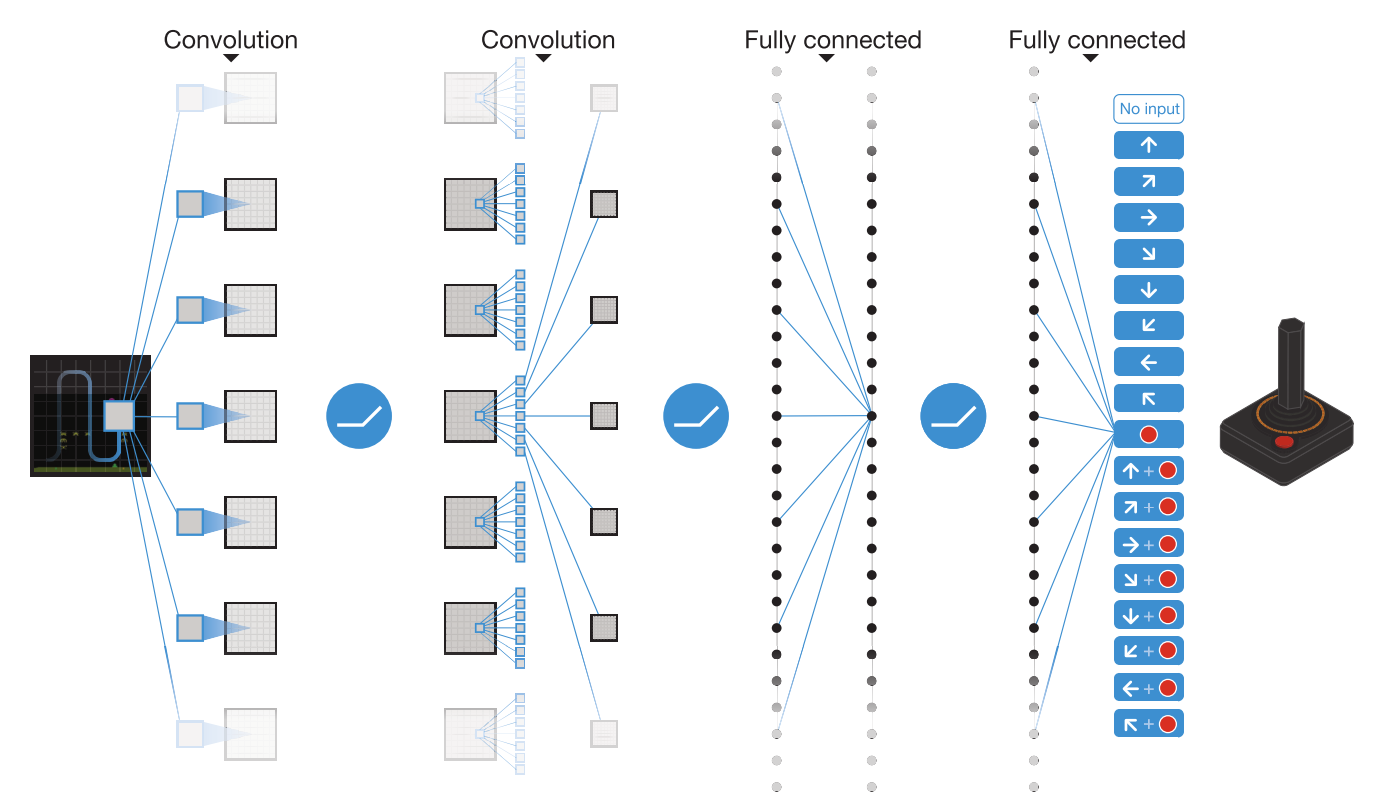
\includegraphics[width=\textwidth]{dqn}
		\caption[Cấu trúc mạng ``Deep Q-Network'']{Hình mô tả cấu trúc mạng ``Deep Q-Network'' \cite{mnihdqn2015}.
		Các tầng ẩn đầu tiên là tầng tích chập với hàm kích hoạt ``rectified linear''.
		Tầng ẩn tiếp theo là tầng ``fully-connected'' có nhiệm vụ tổng hợp đặc trưng trên toàn ảnh của tầng trước.
		Tầng output cũng là tầng ``fully-connected'' trả về kết quả là giá trị của từng hành động ứng với trạng thái đầu vào.
		Tầng output không có hàm kích hoạt.}
		\label{fig_dqn_nature}
	\end{figure}

%-----------------------------------------------------------------------------
\subsection{Kỹ thuật làm tăng tính ổn định}
	Đặc điểm của thuật toán ``Q-learning'' khi kết hợp với xấp xỉ hàm đó là thuật toán không chắc sẽ hội tụ \cite{sutton1998introduction}.
	Hội tụ ở đây ý chỉ sau một số bước cập nhật hữu hạn, giá trị hành động của trạng thái sẽ hội tụ về giá trị nhất định.
	Do đặc điểm này, nếu ta huấn luyện mạng nơ-ron bằng thuật toán SGD thông thường thì nhiều khả năng ``Q-learning'' sẽ không hội tụ dẫn đến chính sách tương ứng sẽ không được tốt.
	Để giải quyết vấn đề này, chúng em áp dụng hai kỹ thuật giúp tăng tính ổn định và khả năng hội tụ: kỹ thuật ``Experience replay'' \cite{lin1993reinforcement} và kỹ thuật cố định ``Q-target'' \cite{mnih2013playing}.
	
\subsubsection*{``Experience replay''}
	Thuật toán ``Q-learning'' kết hợp với xấp xỉ hàm cho phép ta học ``online'': sau mỗi bước tương tác với môi trường và nhận được dữ liệu mới, ta có thể cập nhật ngay bộ trọng số mạng nơ-ron.
	Tuy nhiên, cách học này có thể gây ra vấn đề không hội tụ.
	Lý do là các mẫu dữ liệu liên tiếp nhau thường có tương quan (correlation) với nhau rất lớn.
	Ngoài ra, các mẫu dữ liệu phía sau bị ảnh hưởng bởi chính sách (tương ứng với bộ trọng số mạng nơ-ron) ngay trước đó.
	Ví dụ như chính sách hiện tại là ``luôn qua trái'' thì các mẫu dữ liệu liên tiếp sẽ lấy từ phân bố ``qua trái''.
	Khi chính sách thay đổi sang ``luôn qua phải'' thì tất cả các mẫu dữ liệu mới sẽ lấy từ phân bố ``qua phải''.
	Khi các mẫu dữ liệu có tương quan lớn và phân bố dữ liệu thay đổi nhanh thì ``Q-learning'' sẽ khó hội tụ \cite{mnihdqn2015}.
	
	Kỹ thuật ``experience replay'' \cite{lin1993reinforcement} giải quyết vấn đề này bằng cách lưu trữ lại một tập các mẫu dữ liệu nhận được gần đây nhất.
	Sau đó, mỗi lần muốn cập nhật bộ trọng số, ta chỉ việc lấy ngẫu nhiên một ``mini-batch'' từ tập dữ liệu này để học.
	Ý tưởng của kỹ thuật này giống như việc ta ``gợi nhớ'' lại các kinh nghiệm đã có từ trước đó và học lại từ chúng.
	Cách làm này cũng mang tính ``củng cố'' lại những kinh nghiệm mà hệ thống học được trong quá khứ.
	Do việc lấy ngẫu nhiên nên các mẫu dữ liệu trong ``mini-batch'' sẽ không còn tương quan lớn với nhau.
	Ngoài ra, việc lưu trữ lại giúp các mẫu dữ liệu có thể được học lại nhiều lần.
	Điều này giúp hệ thống học được nhiều hơn mà không phải tương tác với môi trường quá nhiều.
	
\subsubsection*{Cố định ``Q-target''}
	Mỗi khi mạng nơ-ron được cập nhật bộ trọng số thì chính sách hiện tại sẽ thay đổi.
	Khi chính sách thay đổi thì hàm $q_{\pi}$ mục tiêu cũng thay đổi theo.
	Thực tế cho thấy, việc thay đổi nhỏ của bộ trọng số sẽ gây ra thay đổi lớn của chính sách \cite{mnih2013playing}.
	Để thấy được điều này, ta có thể thay đổi trọng số ở những tầng đầu tiên của mạng nơ-ron.
	Khi đó, trọng số này sẽ ảnh hưởng dây chuyền đến những tầng sau làm cho output của mạng nơ-ron bị thay đổi nhiều.
	Do vậy, mỗi khi cập nhật bộ trọng số, hàm mục tiêu $q_{\pi}$ tại một bộ trạng thái $s$ và hành động $a$ nhiều khả năng sẽ thay đổi lớn.
	Do giá trị mục tiêu của việc xấp xỉ hàm thay đổi quá nhiều và liên tục, mạng nơ-ron có thể không xấp xỉ được hàm giá trị như ta mong muốn.
	
	Một kỹ thuật được đề xuất bởi \cite{mnihdqn2015} có tên \textbf{cố định ``Q-target''} (fix Q-target) nhằm giải quyết vấn đề này.
	Thay vì thay đổi giá trị mục tiêu một cách liên tục, ta có thể cố định lại hàm mục tiêu $q_{\pi}$ trong một số bước cập nhật trọng số để mạng nơ-ron xấp xỉ tốt hàm này.
	Sau một khoảng thời gian, ta mới thay đổi hàm mục tiêu thành hàm ứng với chính sách hiện tại.
	Các lần cập nhật trọng số tiếp theo lại tiếp tục cố gắng xấp xỉ tốt hàm mục tiêu mới.
	Quá trình này được lặp lại nhiều lần để hàm mục tiêu cuối cùng mà ta có cũng chính là hàm giá trị tối ưu.
	
	Để có cái nhìn trực quan hơn về kỹ thuật này, ta có thể lấy ví dụ về việc xây một căn nhà.
	Do quá trình thiết kế ban đầu chưa tính trước đến những trường hợp phát sinh (như thiếu vật liệu, thợ không đủ trình độ...) trong lúc xây dựng nên ta phải điều chỉnh thiết kế lại liên tục.
	Ta có thể vừa xây dựng căn nhà (ứng với việc thay đổi trọng số mạng nơ-ron) vừa điều chỉnh lại thiết kế căn nhà cho phù hợp (ứng với việc thay đổi chính sách mục tiêu).
	Tuy nhiên, khi thiết kế căn nhà thay đổi quá nhanh và liên tục thì việc xây dựng sẽ gặp nhiều khó khăn và có khả năng khi hoàn thành kết quả sẽ không tốt.
	Kỹ thuật cố định ``Q-target'' tương tự với việc ta cố gắng xây dựng hoàn tất một phần của căn nhà (tức xấp xỉ tốt hàm giá trị một chính sách cũ) trước khi thay đổi thiết kế.
	Cứ như vậy, mỗi khi hoàn tất một phần, ta thay đổi thiết kế (ứng với việc thay đổi hàm mục tiêu) rồi lại xây dựng tiếp.
	Cách làm này giống như tạo dựng một số các ``điểm kiểm soát'' (checkpoint) với những mục tiêu xác định.
	Do các ``điểm kiểm soát'' này cố định nên việc thay đổi kiến trúc căn nhà sẽ không quá nhiều, dẫn đến quá trình xây dựng sẽ dễ dàng đạt được mục tiêu hơn.
	
	Tuy nhiên, kỹ thuật này dẫn đến một vấn đề là ta cần phải thay đổi hàm mục tiêu sau bao nhiêu lần cập nhật trọng số mạng nơ-ron (tức tần suất thay đổi hàm mục tiêu)?
	Nếu tần suất quá cao (tức thay đổi hàm quá nhiều) thì kỹ thuật này không mang lại được nhiều hiệu quả.
	Nếu tần suất quá thấp (tức ít khi thay đổi hàm mục tiêu) thì việc học sẽ rất chậm do ta phải cập nhật trọng số rất nhiều để xấp xỉ một hàm giá trị cũ; khi cập nhật hàm mục tiêu thì chính sách mới chỉ tốt lên một chút so với chính sách cũ.
	Vì vậy, ta cần phải chọn một giá trị vừa phải, phù hợp với bài toán tự động chơi game.

%-----------------------------------------------------------------------------
\subsection{Vấn đề đánh giá quá cao của thuật toán ``Q-learning''}
	Thuật toán ``Q-learning'' thực hiện việc lấy $\max$ giá trị các hành động của trạng thái tiếp theo.
	Nhắc lại công thức cập nhật của ``Q-learning'' là:
	\begin{equation}
		\theta_{t+1} = \theta_t - \alpha \left[ R_{t+1} + \gamma \max_{a}\hat{q}(S, a;\theta_t) - \hat{q}(S,A;\theta_t) \right] \nabla_{\theta_t} \hat{q}(S, A;\theta_t)	
	\end{equation}
	Nhờ việc lấy $\max$ mà thuật toán ``Q-learning'' hội tụ nhanh hơn \cite{sutton1998introduction}: ta luôn ước lượng giá trị của trạng thái tiếp theo dựa vào hành động tốt nhất tại đó.
	Đây có thể hiểu là một cách nhìn ``lạc quan'' về tương lai: nếu có nhiều trường hợp tốt, xấu khác nhau thì ta luôn giả sử điều tốt nhất sẽ xảy ra.
	Tuy việc giả sử này có thể không đúng trong mọi tình huống, do các trạng thái tiếp theo sau đó cũng được cập nhật lại giá trị nên thuật toán ``Q-learning'' vẫn hội tụ chính xác về chính sách tối ưu.
	
	Rõ ràng là cách nhìn ``lạc quan'' này cũng có điểm xấu: ta sẽ có cái nhìn quá ``lạc quan'' (optimistic) về tương lại và dễ dẫn đến khả năng đánh giá quá cao (overestimation) giá trị của trạng thái kế tiếp.
	Nhất là khi áp dụng xấp xỉ hàm, giá trị ước lượng hiện tại của mạng nơ-ron chưa được chính xác.
	Khi đó nếu mạng nơ-ron ước lượng cao hơn giá trị thật sự thì vấn đề đánh giá quá cao sẽ xảy ra nhiều hơn.
	Mặc dù vậy, ta vẫn cần đặt ra câu hỏi: liệu việc đánh giá quá cao có gây ảnh hưởng đến kết quả của chính sách cuối cùng hay không?
	Rõ ràng là nếu tất cả hành động đều bị đánh giá quá cao (ví dụ như tăng một lượng bằng nhau $C$) thì việc lựa chọn hành động không bị ảnh hưởng (do ta vẫn chọn hành động tốt nhất bằng cách tham lam).
	Tuy nhiên, thuật toán ``Q-learning'' với xấp xỉ hàm gặp hiện tượng đánh giá quá cao không đồng đều \cite{van2015deep}.
	Điều này làm cho kết quả của một số bài toán cụ thể bị ảnh hưởng lớn.
	Nghiên cứu của \cite{hasselt2010double} cho thấy sai số do môi trường gây ra cũng gây ảnh hưởng đến việc xấp xỉ hàm và gây nên hiện tượng đánh giá quá cao.
	Các nghiên cứu trên cho thấy vấn đề này có ảnh hưởng lớn đến chính sách tìm được của thuật toán ``Q-learning''.
	
	Để khắc phục vấn đề đánh giá quá cao, thuật toán ``Double Q-learning'' \cite{hasselt2010double} ra đời và được áp dụng vào bài toán tự động chơi game \cite{van2015deep}.
	Đây là một thuật toán cải tiến của ``Q-learning'' bằng cách thay đổi lại cách ước lượng giá trị của trạng thái tiếp theo.
	Cụ thể hơn, giá trị này theo ``Q-learning'' là: 
	\begin{equation}
		\label{eq_q_max_target}
		R_{t+1} + \gamma \max_{a}\hat{q}(S_{t+1}, a;\theta)
	\end{equation}
	
	Ta có thể tách việc lấy $\max$ giá trị ra thành hai bước: chọn hành động tối ưu và đánh giá hành động đó.
	Bước chọn hành động được thực hiện bằng cách chọn hành động cho giá trị cao nhất tại trạng thái đó: $a_{*} = \argmax_{a}\hat{q}(S_{t+1}, a;\theta)$.
	Bước đánh giá hành động được thực hiện bằng cách lấy lại giá trị của hành động tốt nhất: $\hat{q}(S_{t+1}, a_{*};\theta)$.
	Ghép hai bước này lại ta có cách ước lượng giá trị của thuật toán ``Q-learning'':
	\begin{equation}
		\label{eq_q_argmax_target}
		R_{t+1} + \gamma \hat{q}(S_{t+1}, \argmax_{a}\hat{q}(S_{t+1}, a;\theta); \theta)
	\end{equation}
	Lưu ý rằng công thức (\ref{eq_q_argmax_target}) chỉ là một cách nhìn khác của công thức (\ref{eq_q_max_target}) và hai công thức này hoàn toàn tương đương nhau.
	
	Thuật toán ``Double Q-learning'' giải quyết vấn đề đánh giá quá cao bằng cách đánh giá hành động tốt nhất bằng hàm giá trị của chính sách khác với chính sách hiện tại.
	Cụ thể hơn, ta cần học hai mạng nơ-ron với hai bộ tham số $\theta$ và $\theta^{-}$.
	Khi cần cập nhật bộ tham số $\theta$ của mạng đầu tiên, ta áp dụng công thức:
	\begin{equation}
		\label{eq_dq_argmax_target}
		R_{t+1} + \gamma \hat{q}(S_{t+1}, \argmax_{a}\hat{q}(S_{t+1}, a;\theta); \theta^{-})
	\end{equation}
	Công thức trên chỉ khác với công thức (\ref{eq_q_argmax_target}) ở chỗ ta đánh giá hành động được chọn bằng một mạng nơ-ron khác.
	Nhờ việc ``phân tách'' (decouple) hai bước trên, ``Double Q-learning'' làm giảm khả năng bị đánh giá quá cao mà ``Q-learning'' gặp phải (\cite{hasselt2010double}).
	Vậy tại sao cách cập nhật này lại không gặp vấn đề nêu trên?
	Trong ``Q-learning'', ta cần tính $\max$ của giá trị của nhiều hành động.
	Do mỗi giá trị hành động tính được đều là xấp xỉ nên sẽ có sai số nhất định (tức sai số giữa giá trị xấp xỉ và giá trị thực $\hat{q}(s, a;\theta) - q_{\pi}(s, a)$).
	Giả sử sai số này là ``uniform'' trong đoạn $[-\epsilon, \epsilon]$ với $\epsilon$ là một giá trị dương nhỏ.
	Khi lấy $\max$ giá trị nhiều hành động lại thì nhiều khả năng hành động được chọn sẽ có sai số dương (do các hành động có sai số âm thì giá trị xấp xỉ bị giảm so với giá trị đúng nên khả năng được chọn thấp hơn).
	Khi càng có nhiều hành động thì khả năng hành động đó có sai số dương lại càng cao hơn.
	Điều này làm cho ``Q-learning'' gặp vấn đề đánh giá quá cao.
	Trong khi với thuật toán ``Double Q-learning'', gọi hành động được chọn theo bộ tham số $\theta$ là $a_{*}$.
	Khi đó, xác suất để $a_{*}$ cũng có sai số dương theo bộ tham số $\theta^{-}$ là thấp (do hai bộ tham số học từ dữ liệu khác nhau).
	Nhờ vậy, việc phân tách hai bước chọn và đánh giá hành động giúp làm giảm vấn đề đánh giá quá cao.
	Xem hình \ref{fig_q_learning_plot} và \ref{fig_double_q_learning_plot} mô tả một ví dụ đơn giản để hiểu hơn về vấn đề đánh giá quá cao trong hai thuật toán ``Q-learning'' và ``Double Q-learning''.
	\begin{figure}
		\centering
		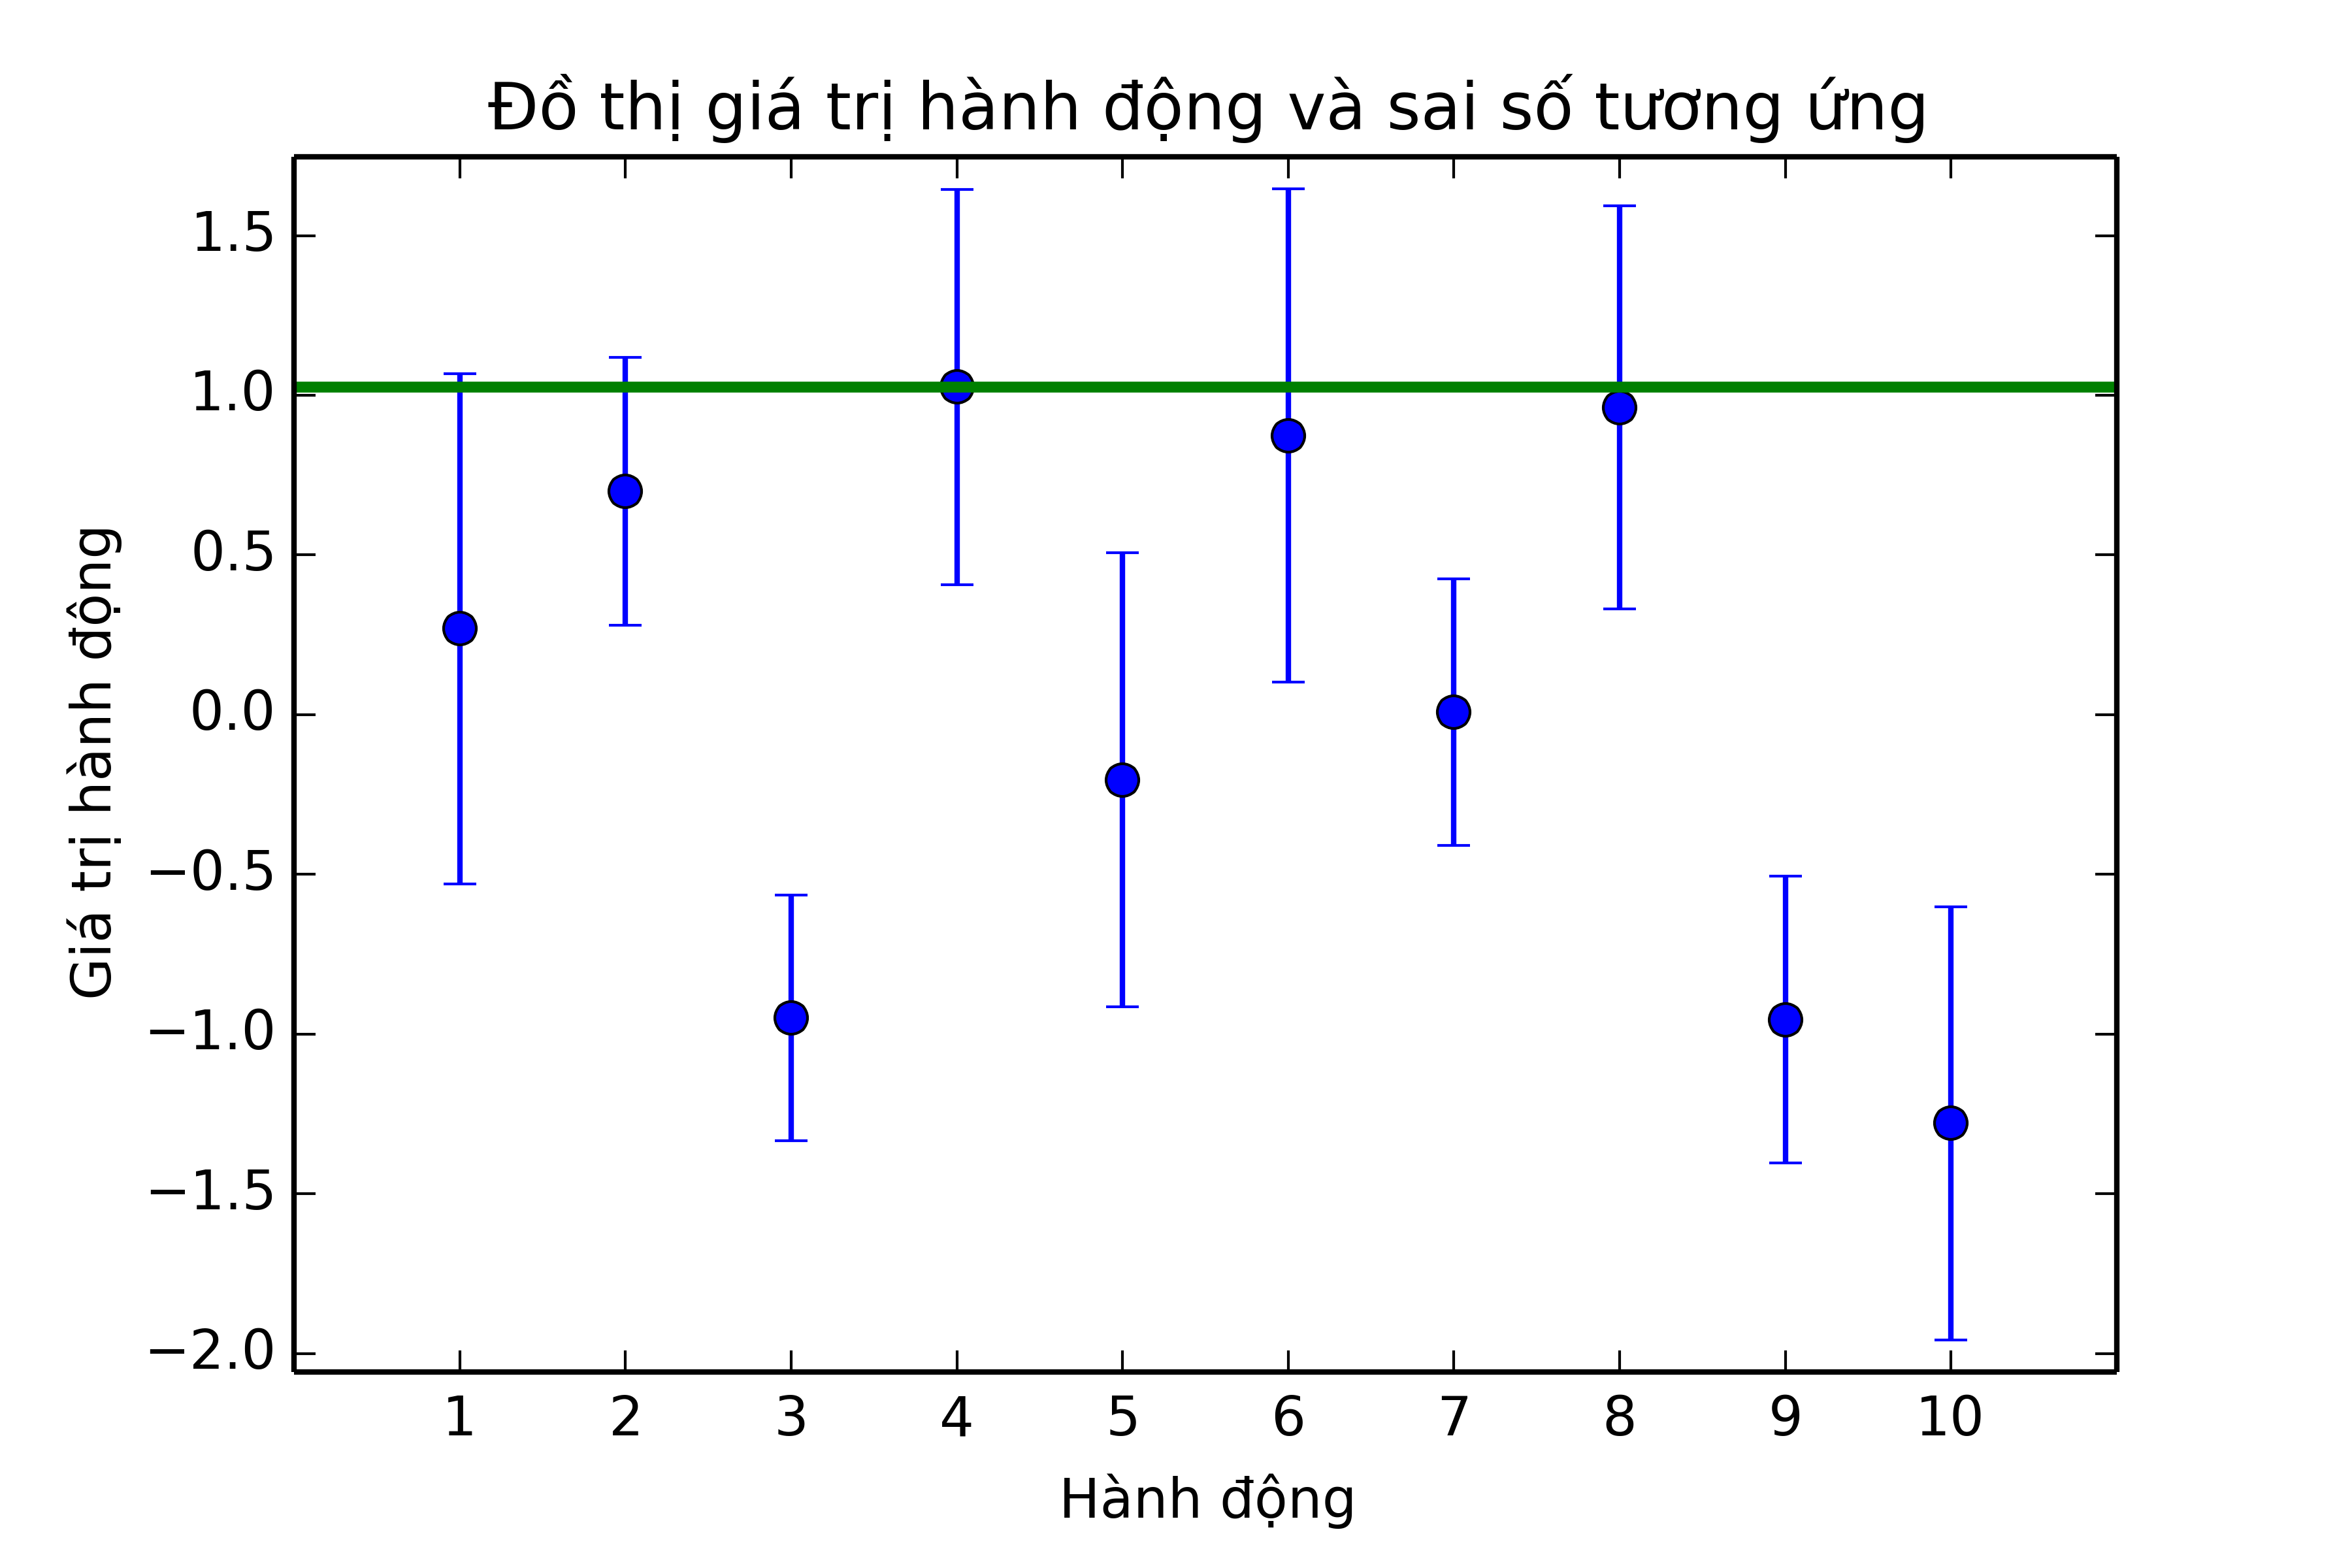
\includegraphics[width=\textwidth]{q_learning}
		\caption[Vấn đề đánh giá quá cao của thuật toán ``Q-learning'']{Hình mô tả vấn đề đánh giá quá cao của thuật toán ``Q-learning''.
		Trục hoành thể hiện mười hành động và trục tung thể hiện giá trị tương ứng.
		Chấm tròn thể hiện giá trị thực sự của từng hành động và các đoạn song song với trục tung thể hiện sai số do quá trình xấp xỉ.
		Đường thẳng nằm ngang thể hiện $\max$ của giá trị thực sự của tất cả các hành động.
		Đây là giá trị đích mong muốn của ``Q-learning''.
		Có nhiều hành động có giá trị xấp xỉ với sai số dương lớn hơn giá trị đích này (hành động 4, 6 và 8) nên khi lấy $\max$ theo ``Q-learning'' thì ta gặp tình trạng đánh giá quá cao.}
		\label{fig_q_learning_plot}
	\end{figure}
	
	\begin{figure}
		\centering
		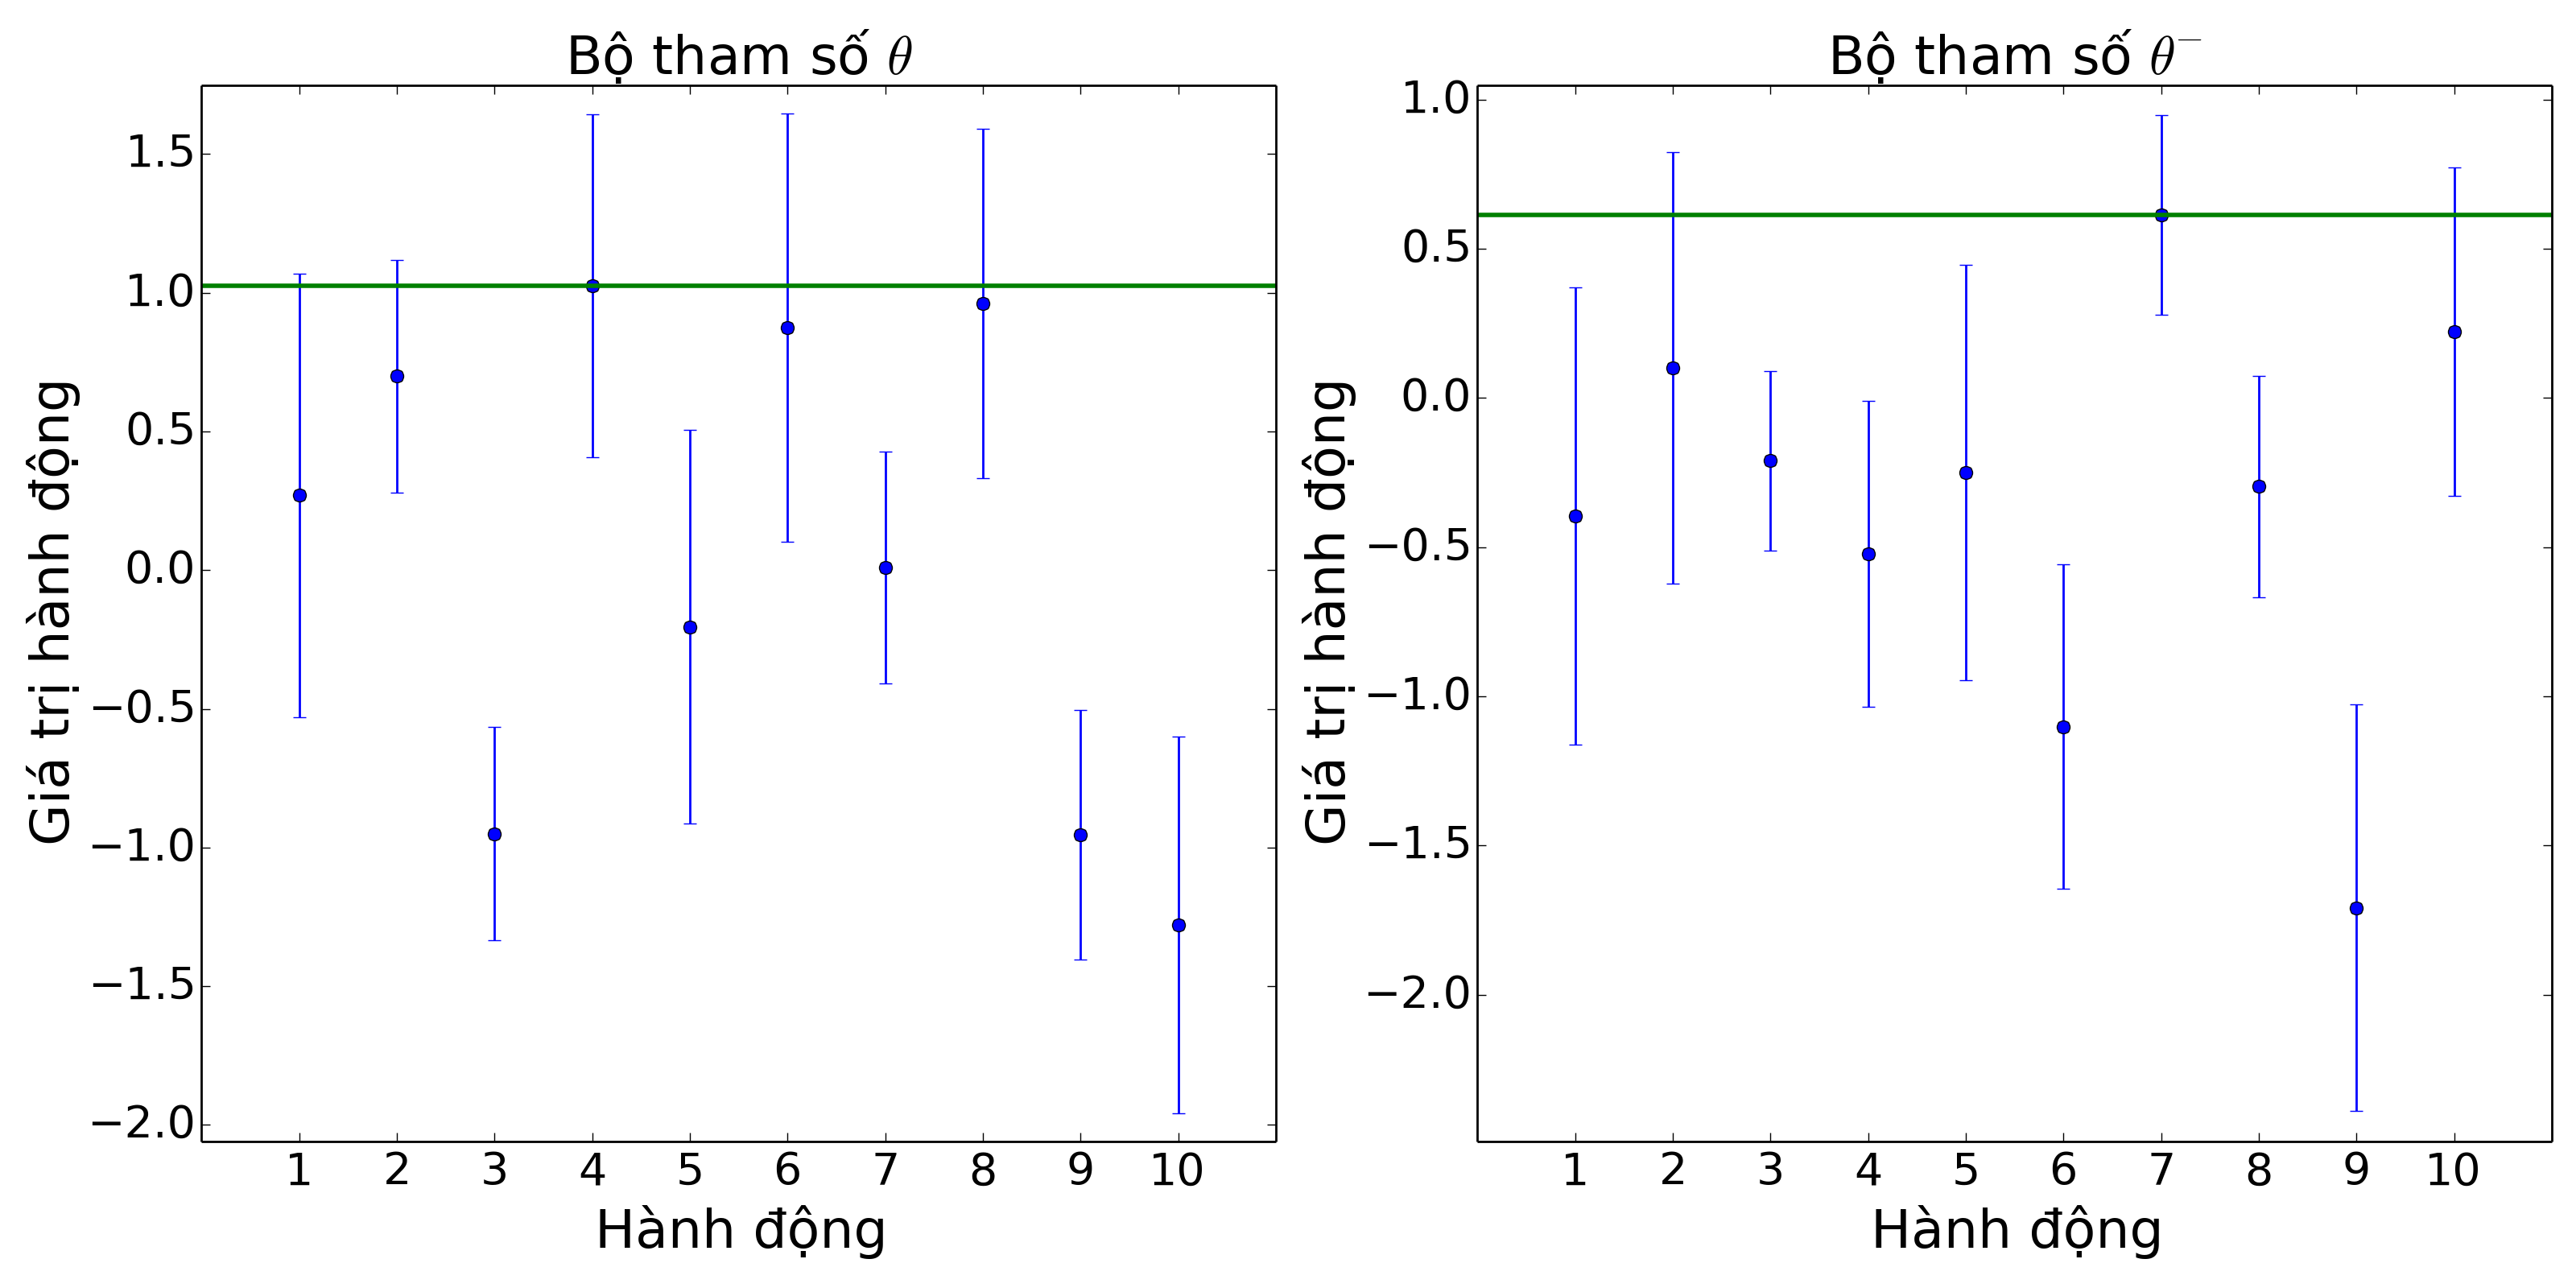
\includegraphics[width=\textwidth]{double_q_learning}
		\caption[Cách giải quyết vấn đề đánh giá quá cao của thuật toán ``Double Q-learning'']{Hình mô tả cách giải quyết vấn đề đánh giá quá cao của thuật toán ``Double Q-learning''.
		Đồ thị bên trái thể hiện giá trị hành động được xấp xỉ theo bộ tham số $\theta$; đồ thị bên phải là giá trị hành động theo bộ tham số $\theta^{-}$.
		Khi chọn hành động theo bộ tham số $\theta$, nhiều khả năng ta sẽ chọn hành động 4, 6 hoặc 8.
		Tuy nhiên, theo bộ tham số $\theta^{-}$ thì các hành động này lại không phải là những hành động có giá trị xấp xỉ cao nhất.
		Nhờ việc lựa chọn và đánh giá hành động một cách độc lập như vậy mà thuật toán ``Double Q-learning'' không gặp vấn đề đánh giá quá cao.}
		\label{fig_double_q_learning_plot}
	\end{figure}
	